% !TeX spellcheck = de_DE
\section{Strategie}
\subsection{Generische Wettbewerbsstrategien}
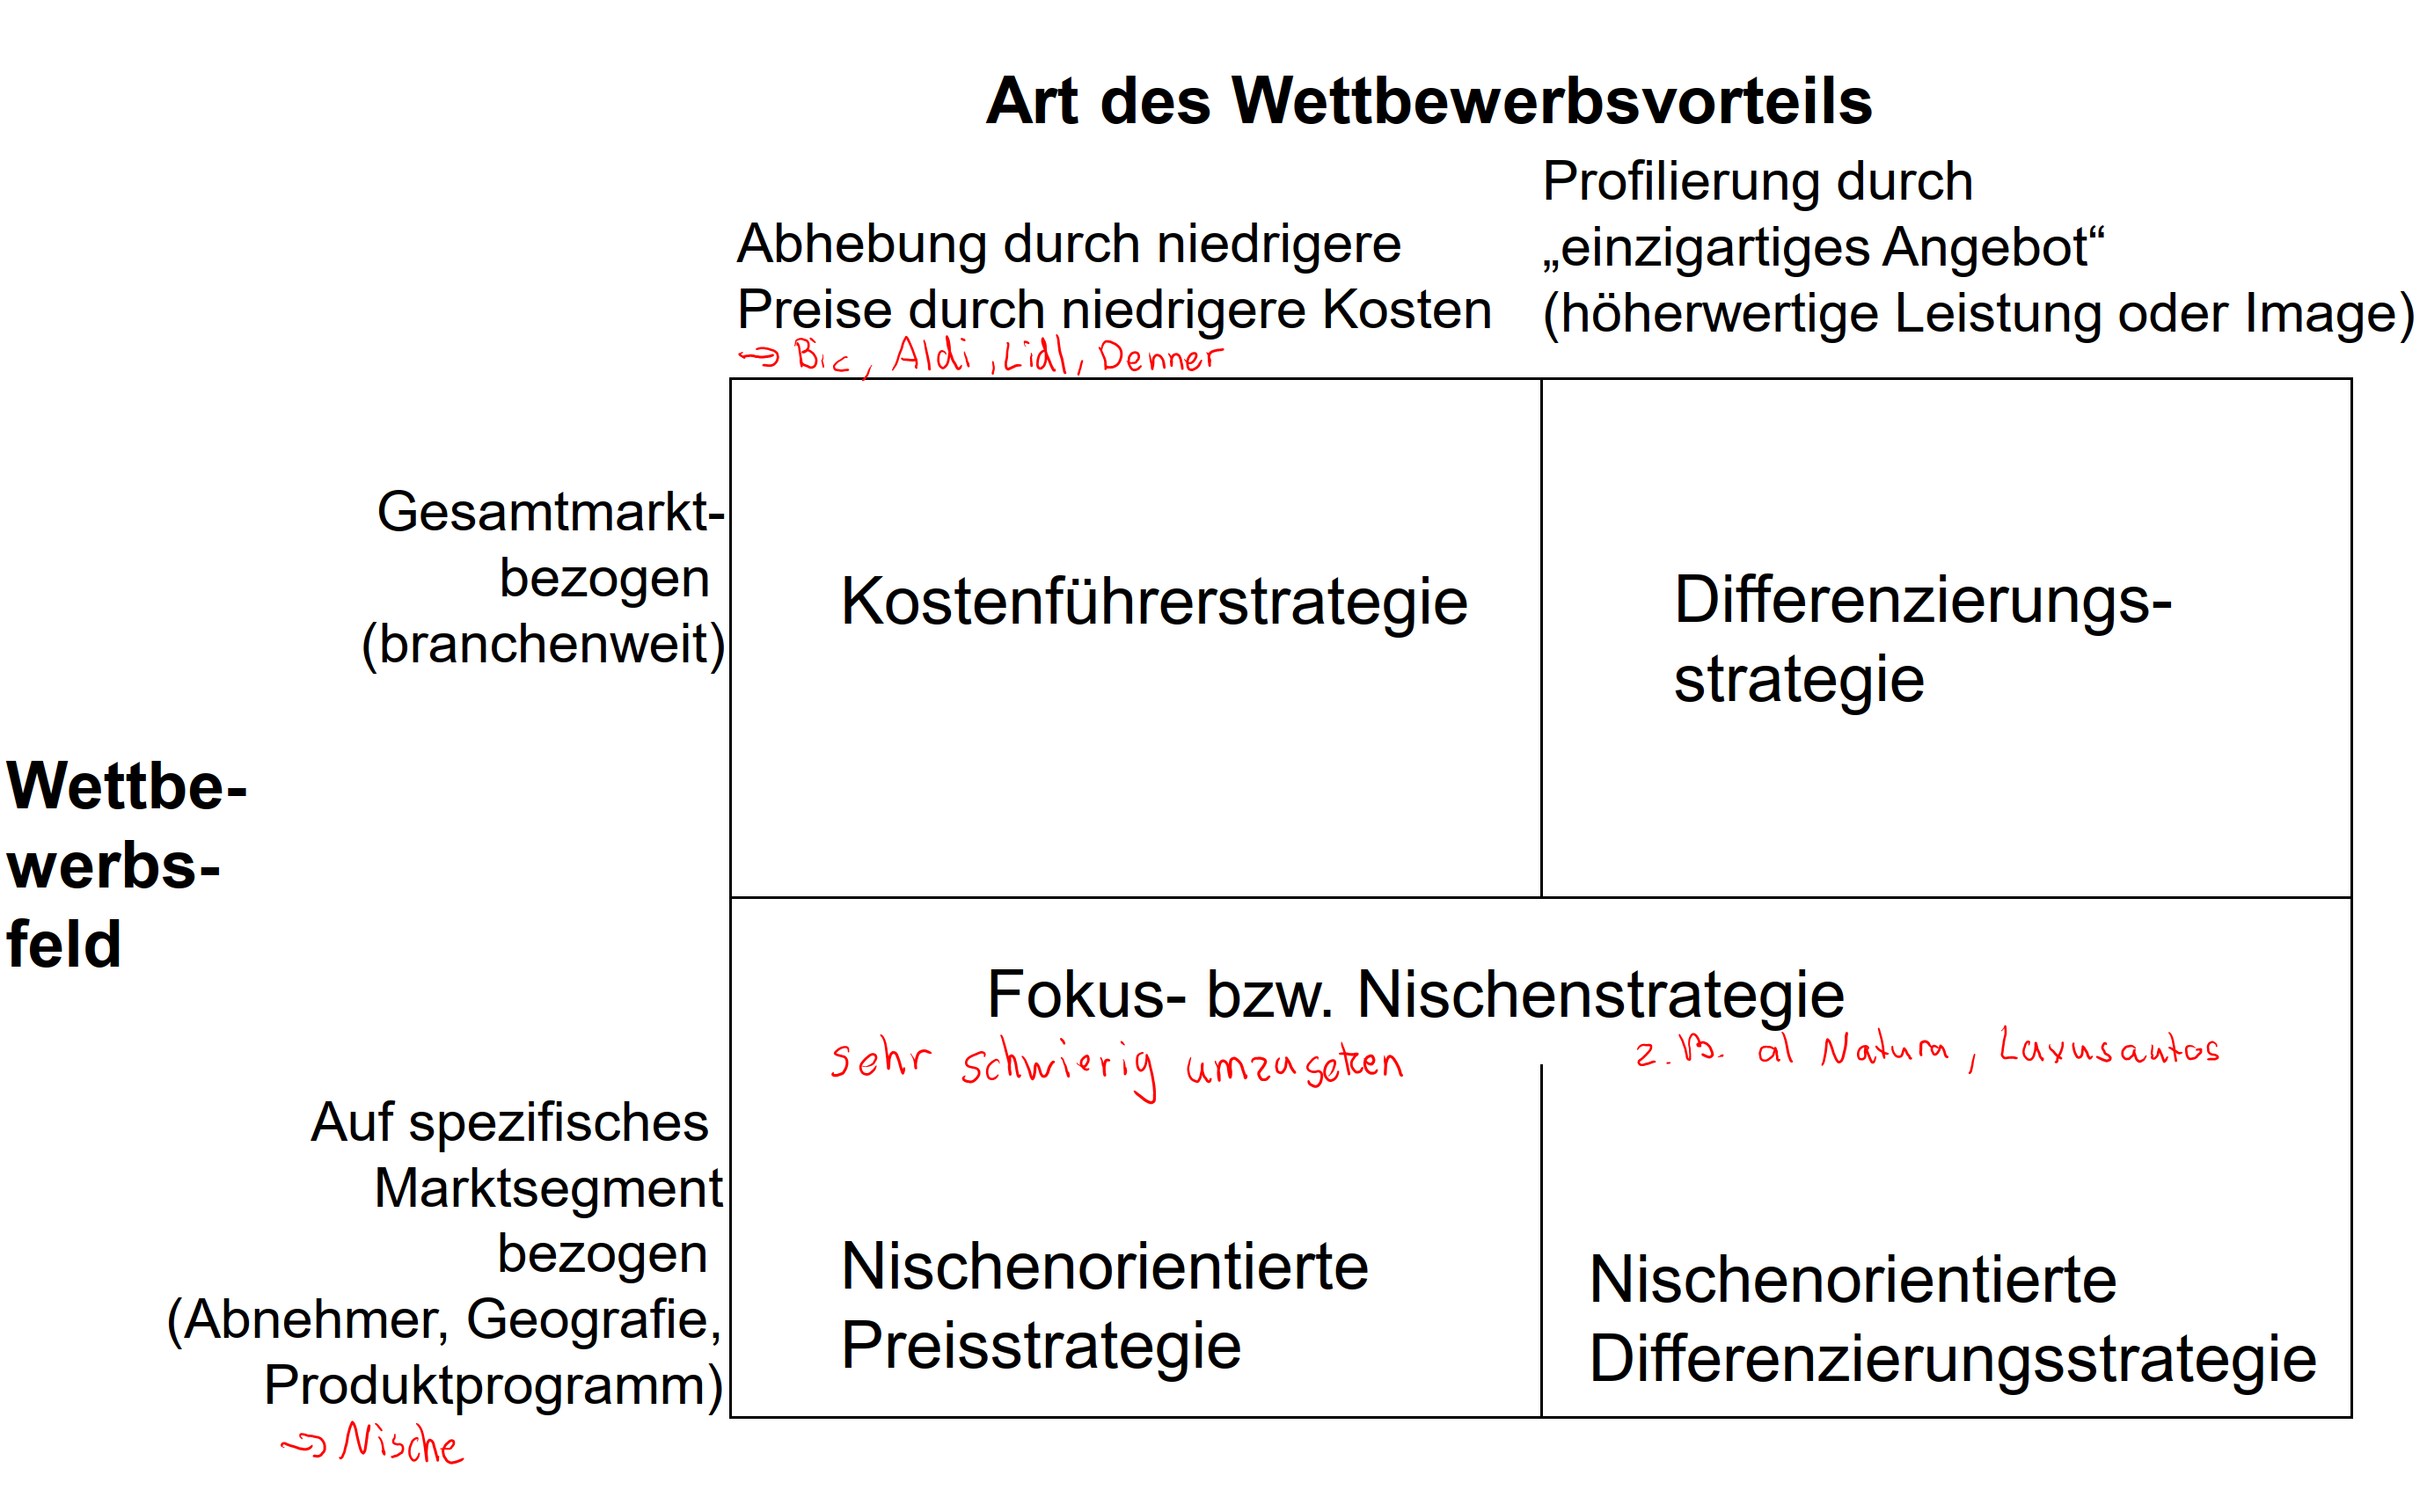
\includegraphics[width=0.5\linewidth]{images/wettbewerbsstrategie}

\subsubsection{Kostenführer}
Kostenführer ist das Unternehmen, das seine Leistungen am günstigsten herstellen und liefern kann.
\begin{itemize}
	\item Strategie kann durch Prozessoptimierung, bewusstes Rationalisieren oder auch Vorhandensein eines natürlichen Vorteils (z.B. günstiger Standort) erreicht werden.
	\item Risiken: mangelnde Flexibilität und Innovationsfeindlichkeit (auf Effizient ausgelegtes System).
	\item Beispiele: Aldi oder Denner im Detaillhandel oder Hyundai in der Autoindustrie.
\end{itemize}

\textbf{Return of Investment:} 30.2 \% (branchenweit), 23.7 \% (segmentspezifisch)

\paragraph{Voraussetzungen und Risiken}
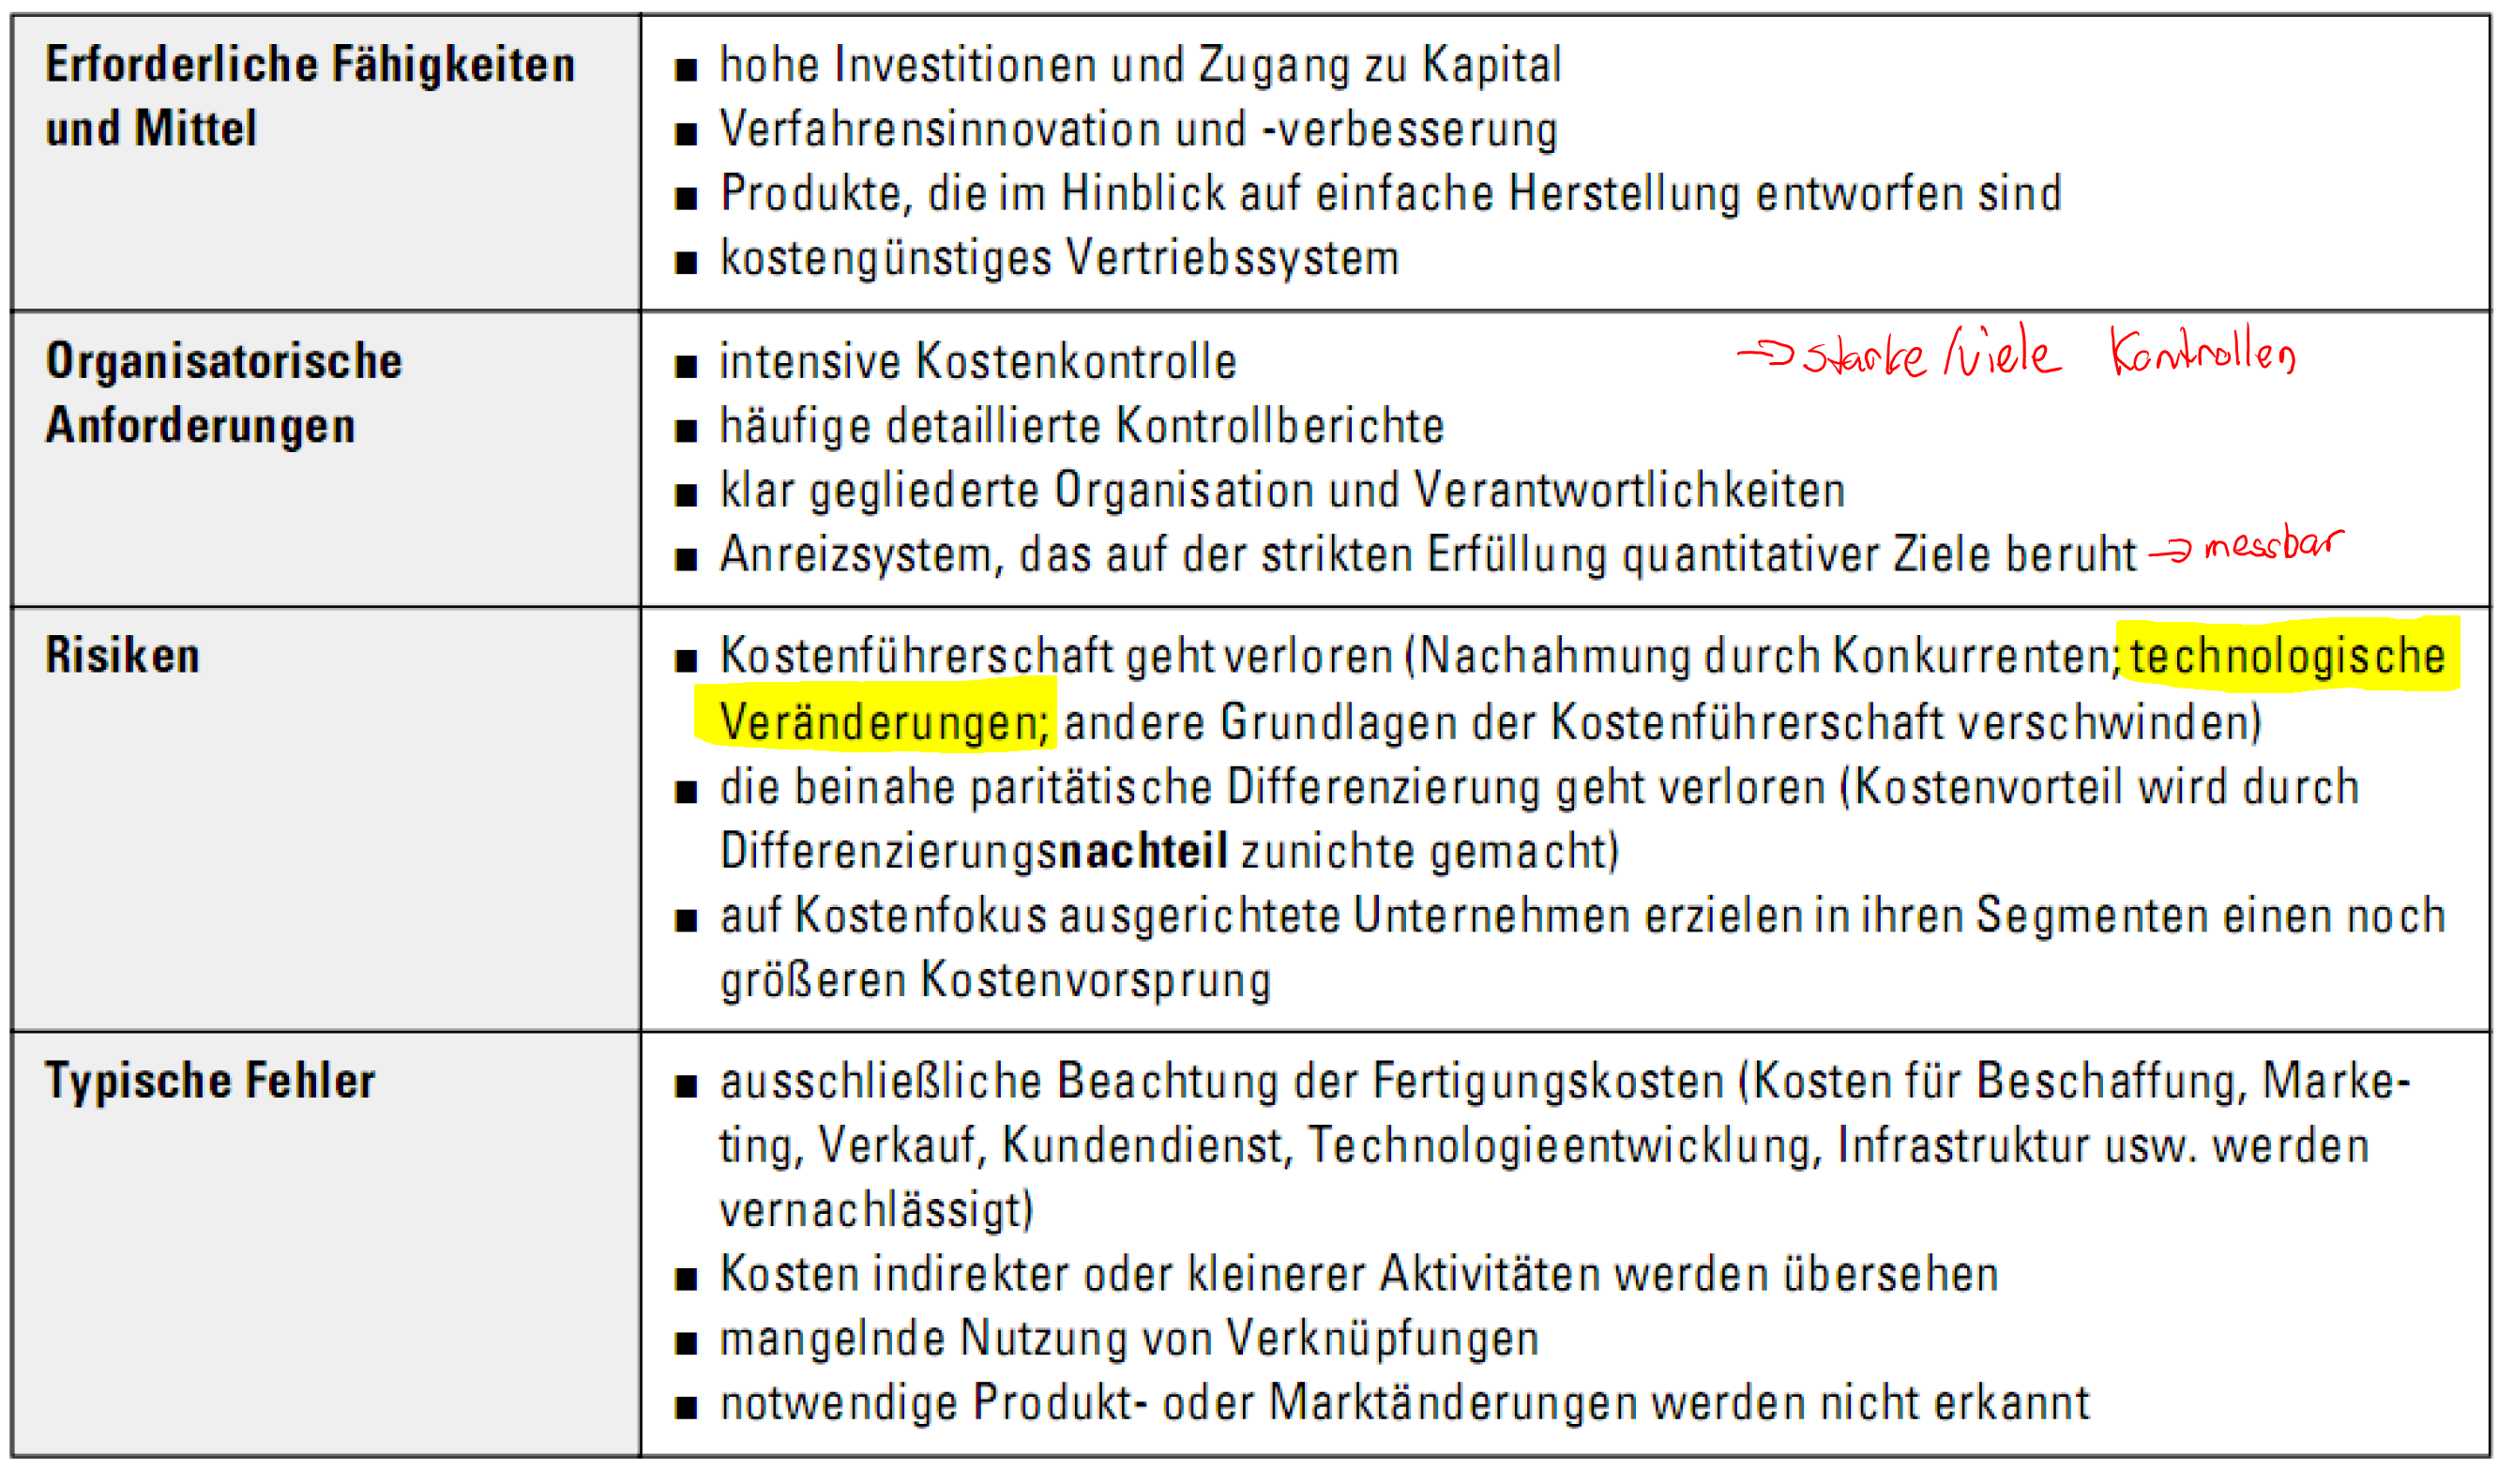
\includegraphics[width=0.7\linewidth]{images/risiko_kostenfuehrerschaft}

\subsubsection{Differenzierung}
Differenzierung bezweckt, das Leistungsangebot eines Unternehmens so zu gestalten, dass es sich möglichst deutlich von den Angeboten der Konkurrenten unterscheidet. Ziel ist Einzigartigkeit innerhalb der Branche. Unterscheidungsmerkmale befriedigen die Bedürfnisse der Kunden optimal, sind nicht einfach zu kopieren und Kunde ist bereit, dafür höheren Preis zu bezahlen.

\textbf{Beispiele:}
\begin{itemize}
	\item Markennamen (Nokia™, Coca Cola™, Armani™),
	\item einzigartige Technologien (Google mit neuen Internet-Suchstrategien)
	\item herausragende Produktqualität (z.B. Toyota - Pannentests).
\end{itemize}

\textbf{Return of Investment:} 32.9 \% (branchenweit), 17.0 \% (segmentspezifisch)

\textbf{Risiken:} Vernachlässigung der Kosten und der mögliche Verlust der Differenzierungsvorteile (Nachahmer, Veränderung Kundenbedürfnisse).

\paragraph{Voraussetzungen und Risiken}
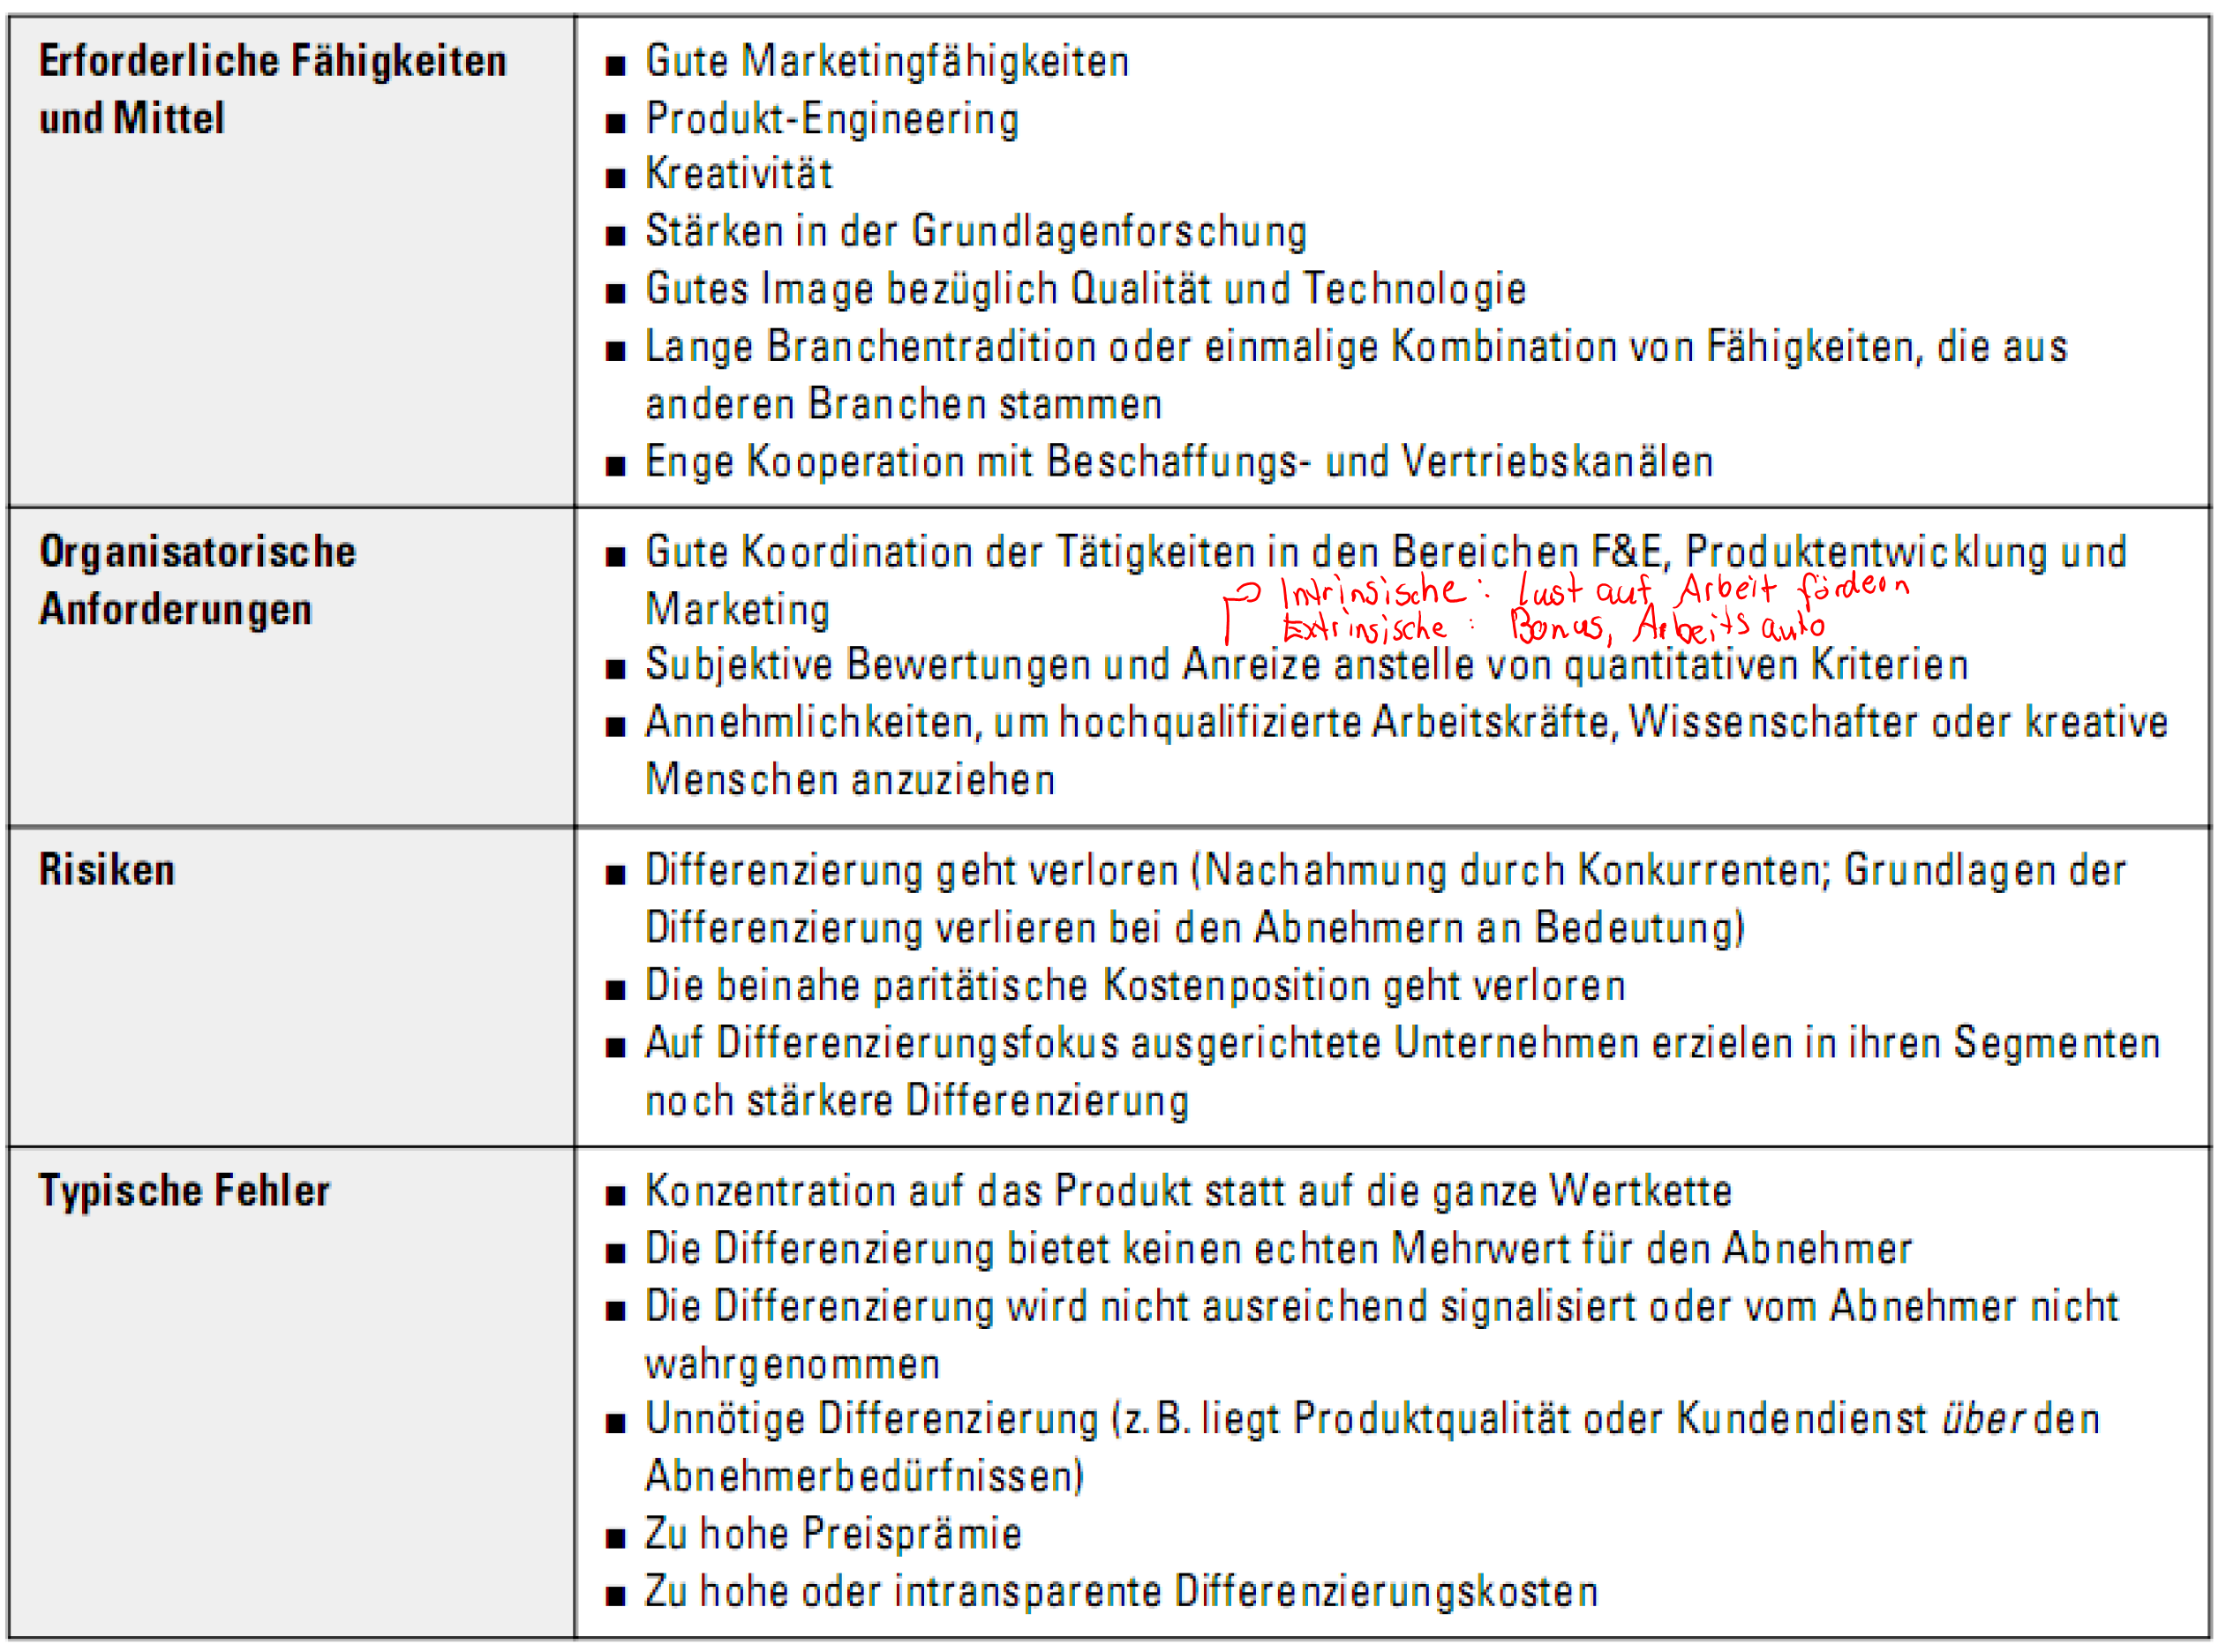
\includegraphics[width=0.7\linewidth]{images/risiko_differenzierung}

\subsubsection{Fokussierung}
Fokussierung (oder Nischenstrategie) zielt mit dem Leistungsangebot
\begin{itemize}
	\item auf eine ganz bestimmte \textbf{Kundengruppe} (Übergrössen in der Bekleidungsindustrie),
	\item auf ein Segment in einer \textbf{Produktlinie} (Wanderferien in der Tourismusbranche),
	\item auf einen stark eingegrenzten \textbf{geografischen Markt} (nur Ferien auf Madeira).
\end{itemize}
Durch Fokussierung wird ein eingegrenzter Markt effizienter und wirkungsvoller bedient; dadurch wird innerhalb eines Teilsegments entweder eine Differenzierung oder eine Kostenführerschaft erreicht.

\subsubsection{Stuck-in-the-Middle}
Keine der drei oberen Strategien. Man befindet sich irgendwo zwischen drin.

\textbf{Return of Investment:} 17.8 \% (branchenweit)

\subsubsection{Doppelstrategie}
Die erfolgreichsten Unternehmen sind jene mit sowohl Differenzierungs- als auch Preisstrategie (Wertkette) (z.B. Ikea, Ryanair).

\textbf{Return of Investment:} 37.8 \% (branchenweit), 31.6 \% (segmentspezifisch)

\subsubsection{Überholstrategien}
Wechselseitiger Einsatz von Kostenstrategie und Differenzierungsstrategie. Z.B. IBM schafft einen Standard (hoher anerkannter Produktwert) und anschliessend werden die Kosten optimiert (niedrige Herstellungskosten). Gleichzeitig versucht der Konkurrent zuerst die Kosten zu optimieren bevor der Produktwert erhöht wird (Überholphase).

\subsection{Branchenweit vs. Segmentspezifisch}
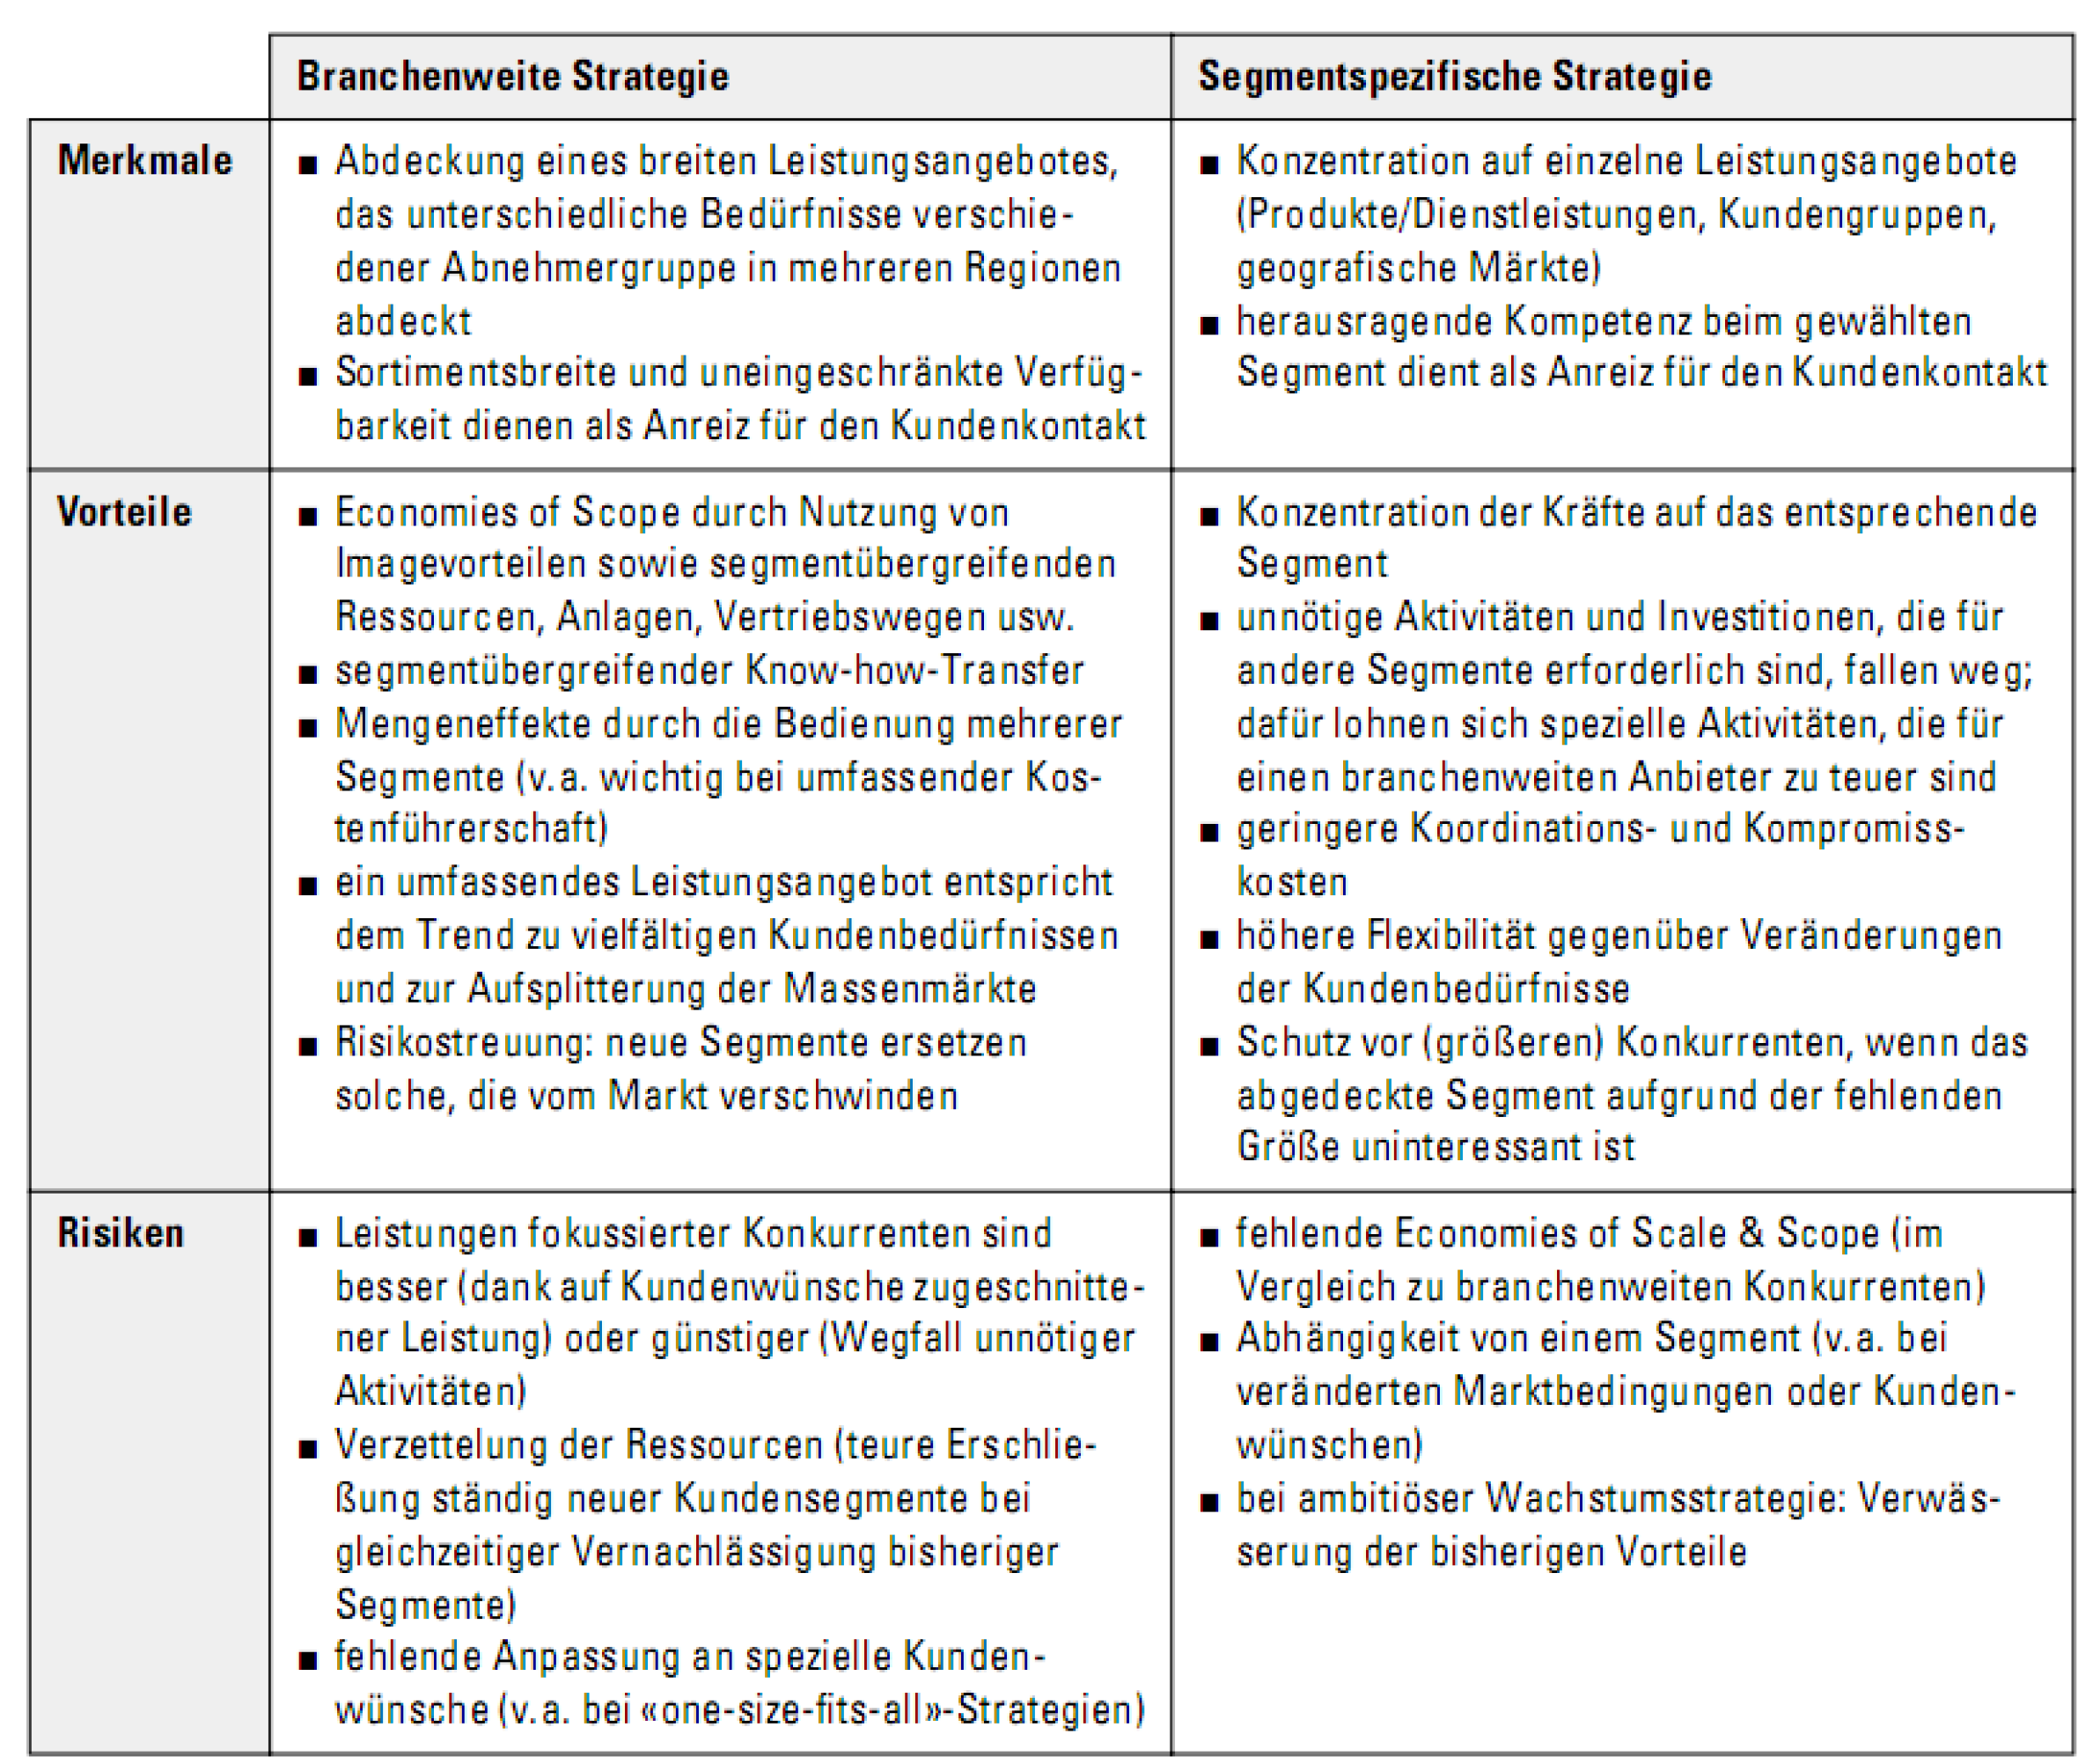
\includegraphics[width=0.7\linewidth]{images/branche_vs_segment}

\subsection{Fünf Wettbewerbskräfte}
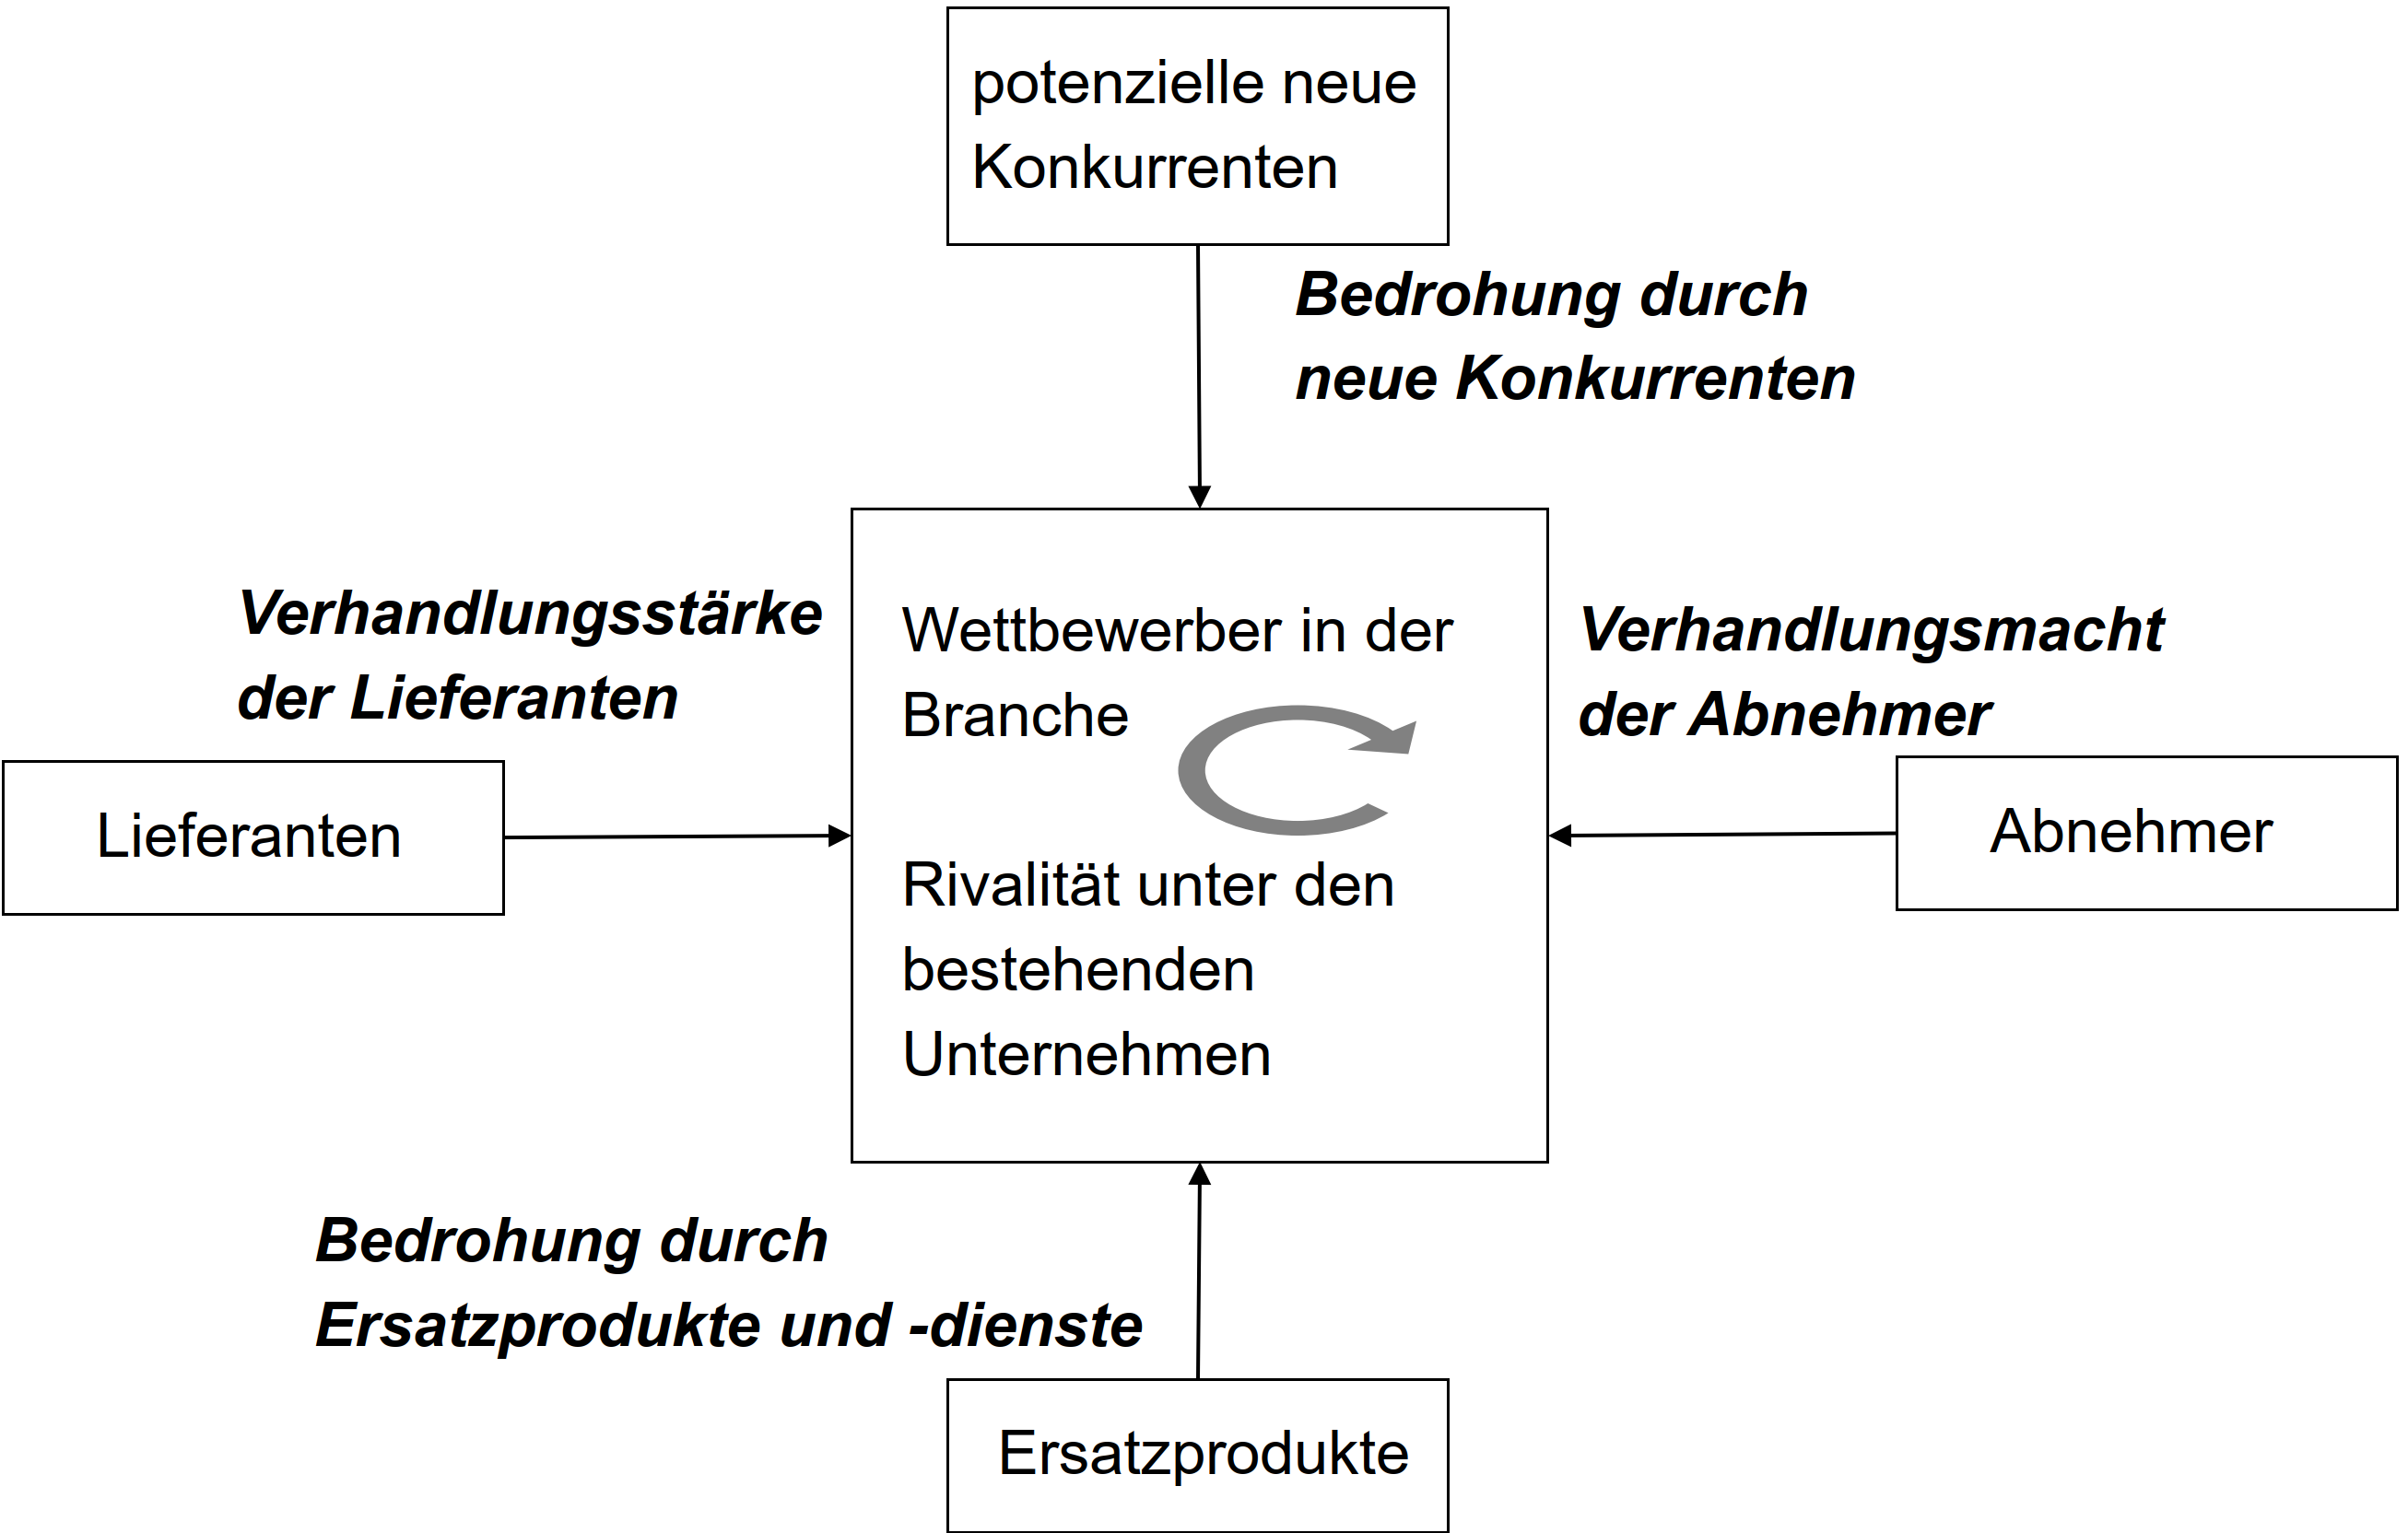
\includegraphics[width=0.5\linewidth]{images/five_forces}

\subsubsection{Neue Konkurrenten}
\textbf{Eintrittsbarrieren:}
\begin{itemize}
	\item Unternehmensseitige Grössenvorteile (Economies of Scale)
	\item Kundenseitige Grössenvorteile (z.B. Ebay, Netzwerke auf Kundenseite)
	\item Wechsel- bzw. Umstellungskosten (z.B. ERP System von SAP, Lock-in-Effect -> gebunden an System)
	\item Kapitalausstattung (Anlageinvestitionen, Kundenkredite etc.)
	\item Andere immanente Vorteile der etablierten Firmen durch Kosten- oder Qualitätsvorteile (z.B. Patente, Marke, Erfahrungsvorsprung etc.)
	\item Zugang zu Vertriebskanälen (z.B. Billigfluglinien via Internet)
	\item Staatliche Regulierungen (Umwelt-/Sicherheitsanforderungen vs. Forschungsförderung)
	\item Vergeltung etablierter Unternehmen (z.B. Preissenkungen, grosse Firmen können teilweise quer subventionieren)
\end{itemize}
Reduzierung der Bedrohung durch neue Konkurrenten durch
\begin{itemize}
	\item Markenimage und Kundenloyalität erhöhen
	\item Patente und Schutzrechte
	\item Markteintrittsbarrieren erhöhen
	\item Allianzen mit komplementären Produkten und Dienstleistungen anbieten
	\item Allianzen mit Lieferanten und Distributionskanälen eingehen (z.B. Deal mit Mindestabnahmemenge)
	\item Effizienzsteigerung der eigenen Leistungserstellung
\end{itemize}

\subsubsection{Zulieferer}
Die Verhandlungsmacht der Zulieferer ist hoch, wenn
\begin{itemize}
	\item je grösser die Konzentration im Markt ihrer Kunden,
	\item sie noch andere Märkte bedienen (Risikostreuung), 
	\item die Kunden hohe Umstellungskosten haben,
	\item ihr Produkt unverzichtbar ist oder gegenüber anderen einen klaren	Vorteil (klare Differenzierung) hat,
	\item ihr Produkt nicht durch Ersatzprodukte bedroht wird,
	\item sie glaubwürdig mit Vorwärtsintegration drohen können.
\end{itemize}

\subsubsection{Käufer}
Die Verhandlungsmacht der Käufer ist hoch, wenn
\begin{itemize}
	\item ihre Lieferanten hohe Fixkosten haben und auf eine Auslastung der Kapazitäten angewiesen sind,
	\item die Produkte standardisiert, austauschbar und nicht differenziert sind,
	\item die Umstellungskosten gering sind,
	\item die Produkte nicht wichtig für die Qualität oder Leistung des Produktes der Abnehmer sind,
	\item sie glaubhaft mit Rückwärtsintegration drohen können (z.B. Netflix, teilweise Amazon).
\end{itemize}
Intermediäre Kunden gewinnen Marktmacht, wenn sie die Kaufentscheidungen in den nachfolgenden Wertschöpfungsstufen beeinflussen können.

Reduzierung der Verhandlungsmacht der Käufer durch
\begin{itemize}
	\item Partnerschaften
	\item Supply Chain Management
	\item Erhöhung der Kundenloyalität
	\item Anreize und Zusatznutzen für Kunden bieten
	\item Kaufentscheidungen auf andere Einflussfaktoren als den Preis verlagern
	\item Einflussreiche Zwischenhändler übergehen und direkte Beziehungen mit Endkunden aufbauen
\end{itemize}

\subsubsection{Substitute}
Substitute stellen eine Bedrohung dar, wenn
\begin{itemize}
	\item die Produkte die gleiche Funktion erfüllen (z.B. Ski/Snowboard, Linse/Brille),
	\item ein Technologiewandel stattfindet,
	\item besseres Preis-/Leistungsverhältnis geschaffen wird,
	\item Umstellungskosten gering sind.
\end{itemize}

Reduzierung der Bedrohung, indem
\begin{itemize}
	\item Branchenstandards kreiert werden,
	\item Unterschiede zum Substitut hervorgehoben werden (echt oder wahrgenommen)
	\item selbst in den Markt für das Substitut eingetreten wird.
\end{itemize}

\subsubsection{Wettbewerber}
Rivalität unter Wettbewerbern durch
\begin{itemize}
	\item Preisrabatte,
	\item Neue Produkteinführungen,
	\item Werbekampagnen,
	\item Serviceverbesserungen.
\end{itemize}

Intensive Rivalität der Wettbewerber bei
\begin{itemize}
	\item vielen Konkurrenten,
	\item geringem Branchenwachstum,
	\item keinen Umstellungskosten,
	\item hohen Austrittsbarrieren (Liquidationswerte, SGE, Image)
	\item nahezu identischen Produkten (keine Differenzierung)
	\item hohen Fix- und Lagerkosten.
\end{itemize}

\subsection{Strategische Optionen}
Grundlagen für Wettbewerbsstrategien bzw. -vorteil
\begin{itemize}
	\item Preisbasierte Strategien (no frills, niedriger Preis)
	\item Differenzierungsstrategien (hybrid, breit, fokussiert)
\end{itemize}
Strategische Ausrichtung
\begin{itemize}
	\item Marktdurchdringung bzw. Effizienz/Konsolidierung
	\item Produkt/Dienstleistungsentwicklung
	\item Marktentwicklung
	\item Diversifikation
\end{itemize}
Methoden zur Verfolgung einer Strategie
\begin{itemize}
	\item Organische Entwicklung/Wachstum
	\item Fusionen und Übernahmen
	\item Allianzen/Kooperationen
\end{itemize}

\subsection{Ansoff Matrix}
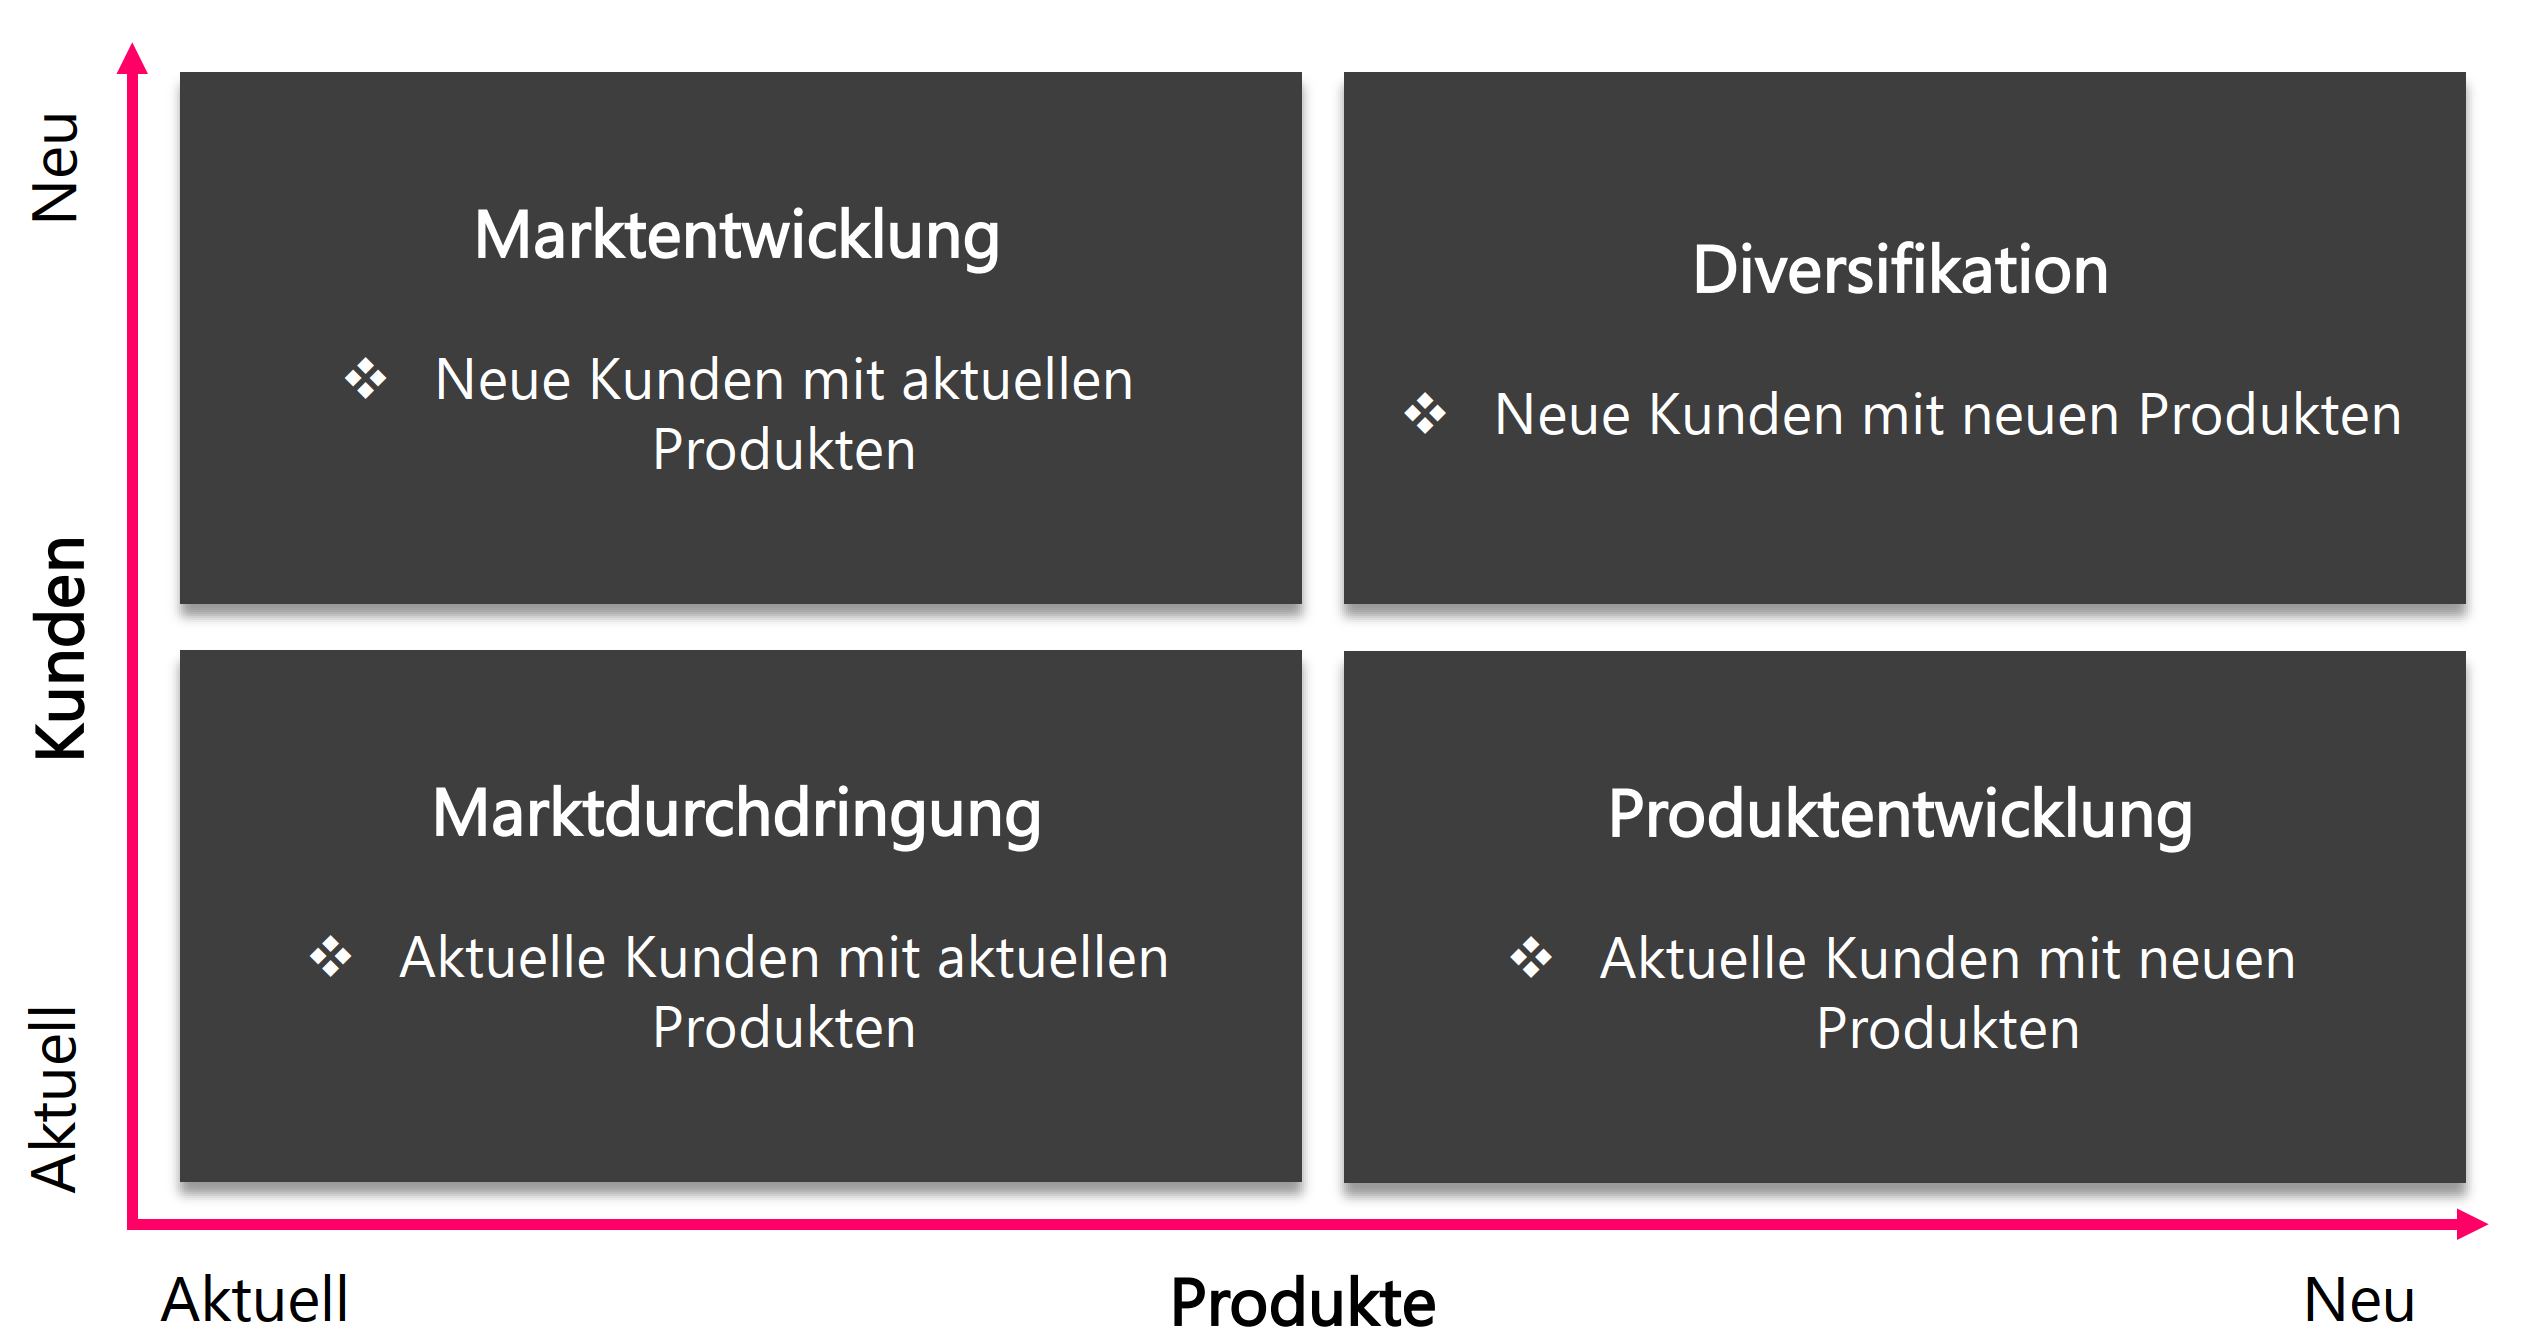
\includegraphics[width=0.5\linewidth]{images/ansoff}

\subsubsection{Marktdurchdringung}
Ausweitung des Marktanteils mittels bestehender Produktpalette (Ich mache das Gleiche was ich schon immer gemacht habe, versuche aber den Markt zu vergrössern)
\begin{itemize}
	\item Baut auf existierenden Fähigkeiten auf
	\item Ausrichtung der Organisation bleibt unverändert
\end{itemize}
Herausforderungen:
\begin{itemize}
	\item Vergeltungsschläge durch Mitbewerber (insb. auf Märkten mit geringem Wachstum) durch Preiskrieg, Marketingkampagnen => hohe Kosten, Variante: Übernahmen von Konkurrenten
	\item Rechtliche Beschränkungen: Kartellbehörden beobachten Marktmacht (z.B. Gaz de France und Suez in Frankreich und Belgien)
\end{itemize}

\paragraph{Konsolidierung}
Unternehmen konzentriert sich auf defensive Weise auf bestehende Märkte und Produkte (keine Wachstumsorientierung)
\begin{itemize}
	\item Verteidigung des bestehendes Marktanteils zum Tragen der Fixkosten (Differenzierung zur Kundenloyalität, Lock-In)
	\item Downsizing bzw. Abstossen bestimmter Geschäftsbereiche (schrumpfende Märkte)
	\item oder Kauf von Konkurrenten in fragmentierten Branchen, in der es meist auch wirtschaftlich abwärts geht (Reduktion von Kapazitäten und Steigerung Marktmacht und Effizienz).
\end{itemize}

\subsubsection{Produktentwicklung}
Unternehmen bieten verbesserte oder neue Produkte auf bestehenden Märkten an (Produktinnovationen, z.B. Walkman, CD, MP3-Player) \\
Teuer und riskant:
\begin{itemize}
	\item Neue strategische Fähigkeiten wie unvertraute Technologien (z.B. Online-Banking nach 2000)
	\item Risiken beim Projektmanagement durch Komplexität und sich verändernde Spezifikationen (z.B. Airbus 380)
\end{itemize}

\subsubsection{Marktentwicklung}
Bereits existierende Produkte werden auf neuen Märkten angeboten
\begin{itemize}
	\item Neue Segmente bzw. Kundengruppen
	\item Neue Anwendungsform/Verwendungszwecke
	\item Neue Regionen bzw. geografische Ausweitung
\end{itemize}
Herausforderungen:
\begin{itemize}
	\item Richtige Koordination der verschiedenen Segmente, Nutzer, Regionen mit all ihren unterschiedlichen Anforderungen.
	\item Produkte müssen oft auch adaptiert werden.
\end{itemize}

\subsubsection{Diversifikation}
Unternehmen weitet Marktabdeckung und Produktprogramm aus.
\begin{itemize}
	\item Verbunden: stützen auf dieselben Fähigkeiten und Wertschöpfungsaktivitäten (z.B. Proctor \& Gamble), horizontal und vertikal
	\item Unverbunden: Neue Aktivitäten haben wenig mit bestehendem Leistungsprogramm gemeinsam (vgl. Mischkonzernstrategie)
\end{itemize}
Gründe:
\begin{itemize}
	\item Steigerung der Effizienz durch Verbundvorteile (Economies of Scope) und Synergien
	\item Fähigkeiten der Unternehmenszentrale ausweiten (dominante Logik)
	\item Steigerung der Marktmacht und Risikostreuung (Quersubventionierung)
\end{itemize}